\section{Kameramodell}
Da das verwendete Fisheye-Objektiv durch seinen großen Blickwinkel stark verzerrt auf den Kamerasensor abbildet, ist eine spezielles Kameramodell zur Rektifizierung der Bilddaten notwendig. Wir haben uns in dieser Arbeit für die Nutzung einer Matlab-Toolbox entschieden  \autocite{OCamCalibOmnidirectionalCamera, scaramuzzaFlexibleTechniqueAccurate2006, scaramuzzaToolboxEasilyCalibrating2006, scaramuzzaOmnidirectionalVisionCalibration2007, rufliAutomaticDetectionCheckerboards2008}. Das in selbiger verwendete Modell und die Anwendung dessen zur Rektifizierung soll nun erleutert werden. 

Die OcamCalib-Toolbox behandelt das Kamerasystem als Einheit, d.h. die Kamera und der Fisheyeobjektivaufsatz (alternativ der konvexe Spiegel) werden zusammen durch einen Parametersatz beschrieben.

Das Modell hat das Ziel, den Zusammenhang zwischen einem Punkt auf dem Bildsensor \gls{lat:camerapoint} mit Koordinaten (u,v) und einem vom optischen Zentrum des Objektivs ausgehenden Vektors nicht festgelegter Länge \gls{lat:cameravector} mit Koordinaten (x,y,z) zu finden.\\

\begin{figure}[H]
  \centering
  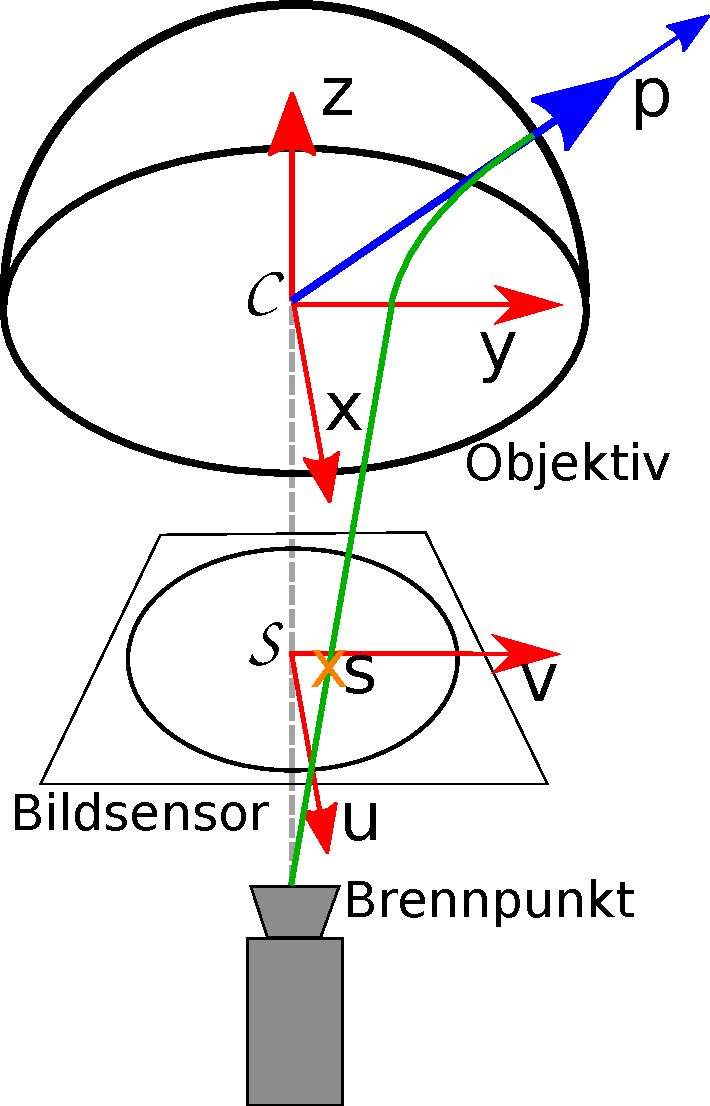
\includegraphics[width=0.5\textwidth]{OCamCalib_Kameramodell}
  \caption{Das Kameramodell der OCamCalib Toolbox}
  \label{fig:kameramodell}
\end{figure}


\subsection{Annahmen}
Im verwendeten Modell werden folgende annahmen gemacht:\\
\begin{itemize}
\item Die verwendete Optik stellt ein zentrales Kamerasystem dar, d.h. alle einfallenden Strahlen, welche sich im Brennpunkt des Objektivs nach der Brechung schneiden (s. grüner Strahlverlauf), schneiden sich auch ungebrochen in einem Punkt (s. blauer Strahlverlauf). Dieser Punkt ist das optische Zentrum des Objektivs und der Koordinatenursprung des Kamerakoordinatensystems xyz.
\item Die Achse des Bildsensors und des Objektivs sind nahezu identisch (s. unterbrochene graue Linie). Das Modell berücksichtigt nur kleine Abweichungen der Rotationen der Achsen.
\item Das Objektiv ist rotationssymetrisch zu seiner Achse.
\item Die Linsenverzerrung wird nicht durch herkömmliche Methoden, sondern durch die Projektionsfunktion f(u,v) berücksichtigt.
\end{itemize}

Da ein Darlegen des Prozesses zur Ermittlung der Parameter den Rahmen dieser Arbeit sprengen würde, wird darauf verzichtet.